\documentclass[tikz,border=10pt]{standalone}
\begin{document}
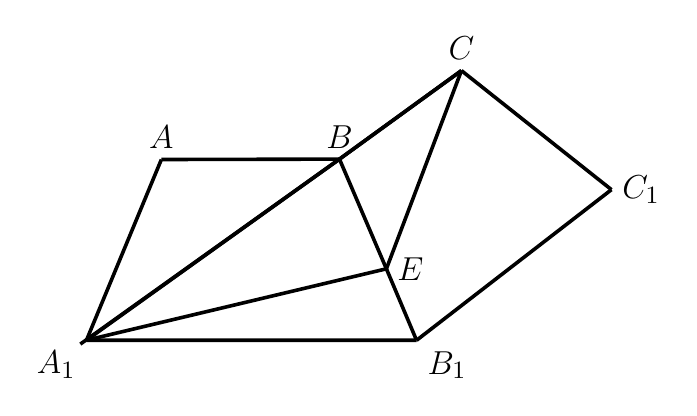
\begin{tikzpicture}[line join=round, line width=1.3pt]
\coordinate (A) at (-2.384,0.622);
\coordinate (B) at (-0.122,0.627);
\coordinate (C) at (1.427,1.751);
\coordinate (GeoTailB) at (-3.413,-1.722);



\coordinate (A1) at (-3.335,-1.673);   
\coordinate (B1) at (0.857,-1.674);    
\coordinate (C1) at (3.332,0.239);     
\coordinate (E)  at (0.474,-0.766);    


\draw (A) -- (B);            
\draw (B) -- (C);            
\draw (B) -- (GeoTailB);     
\draw (A1) -- (A);           
\draw (A1) -- (B);           
\draw (B) -- (C);            
\draw (A1) -- (E);           
\draw (C) -- (E);            
\draw (B) -- (E);            
\draw (E) -- (B1);           
\draw (A1) -- (B1);          
\draw (B1) -- (C1);          
\draw (C) -- (C1);           


\node[above] at (A) {\fontsize{13}{15.6}\selectfont $A$};
\node[above] at (B) {\fontsize{13}{15.6}\selectfont $B$};
\node[above] at (C) {\fontsize{13}{15.6}\selectfont $C$};
\node[right] at (E) {\fontsize{13}{15.6}\selectfont $E$};
\node[below left] at (A1) {\fontsize{13}{15.6}\selectfont $A_1$};
\node[below right] at (B1) {\fontsize{13}{15.6}\selectfont $B_1$};
\node[right] at (C1) {\fontsize{13}{15.6}\selectfont $C_1$};
\end{tikzpicture}
\end{document}